% Chapter 5

\chapter{Evaluation} % Main chapter title

\label{Evaluation} % For referencing the chapter elsewhere, use \ref{Chapter1} 
%----------------------------------------------------------------------------------------
This chapter will present the evaluation and results of the goals that were set in chapter \ref{Introduction}: \textbf{Introduction }.\\
At first, approaches will be explained to evaluate the goals and related work will be presented. After this, the methods are proposed containing the preprocessing steps and the selection of the training and validation sets with respect to the different approaches. In the last step, results are presented and discussed.


%----------------------------------------------------------------------------------------
\section{Approaches}
In this work there were three approaches to analyze the influence of object roles in the haptic search experiment. For all of them supervised machine learning was used resulting in three different classification problems: \\
\begin{enumerate}
	\item \textbf{Classifying data into object categories:} a model was build to classify the five stimuli used in the experiment. At first the model was trained only on the data of objects when they were targets, and second on the data when they were distractors. The performance was measured and compared. The goal was to see if the data would be separable at all and to find a fitting model for it.
	
	\item \textbf{Classifying a single object as either target or distractor:} based on the previous problem, same model was trained separately for each object to classify its data into a target role or a distractor role. 
	
	\item \textbf{Classifying whole data into roles:} in this problem, the model was trained on all data to classify targets and distractors in general. The goal was to see if regardless of the object, data can be separated into target or distractor class.       
\end{enumerate}

Combining the results of all these problems, an answer to the question whether humans explore same objects differently in a haptic search task depending on what the target is should be given. Furthermore an approach to explain the human efficiency could be made by the results. Instead of classifying all explored objects, they distinguish just between two classes, the target object they searched for and a distractor.      
%----------------------------------------------------------------------------------------
\section{Related Work}
This work combines both, object categorization based on their various characteristics and haptic search. Researchers have dealt with the specific task of object classification in previous studies. Since material and functional properties could not be captured because the stimuli used were static and not deformable objects, previous work on shape based classification is perhaps the most related work to the proposed approaches.\\
Schneider et. al. \cite{Schneider} use touch sensors in a manipulation robots fingertips to gain low-resolution intensity images from multiple grasping interactions. They apply a bag-of-words approach and clustering techniques to categorize objects based on haptic feedback. Navarro et. al. presents an approach for haptic recognition and evaluation on multi-fingered robot hands based on extracting key features of tactile and kinesthetic data using clustering \cite{Navarro}. Faldella et. al \cite{Faldella} describes an approach to robotic haptic recognition using an unsupervised Kohonen self-organizing feature map for performing a match-to-sample classification of three-dimensional objects. Pezzementi et. al.views tactile sensor data as images and applies PCA techniques to identify principal components of identified features and clusters them as well as build per-class histograms as class characteristics \cite{Pezzementi}. Gorges et. al. \cite{Gorges} additionally includes passive joints in the tactile sensor system which could help to acquire more information for shape reconstructionn. They use Self-Organizing Maps for identifying haptic key features and a Bayes Classificator for classifying objects. Bhattacharjee et. al. \cite{Bhattacharjee} demonstrate a tactile sensor array covering a robot's forearm to generate haptic time series data during manipulation tasks. They use the processed and dimensionality reduced data to generate feature vectors and classify them with a k-nearest neighbor algorithm for object recognition.
\\\\
Although it is not dealt with categorization of explicit shape features in the previously defined classification problems, the tactile data acquisition, preprocessing and feature extracting used in these works could also be applied for these approaches. Especially parts of the data sampling and preprocessing pipeline from Bhattacharjee et. al. \cite{Bhattacharjee} was found to be well applicable on the data recorded for this work.

%----------------------------------------------------------------------------------------
\section{Methods}
In this section the pipeline is presented that was used for the classification problems of the evaluation. At first the preprocessing steps will be explained that will turn the raw data into feature vectors that can be used for training. Figure \ref{pipeline} depicts the complete experimental protocol. In the second part it will be described how the data sets for training and validation looked like and how they were chosen.

\subsection{Preprocessing and Feature Extraction}
Tactile data was recorded from the glove with a frequency of 150Hz and joint angles at 50Hz. The classification problems were evaluated on both only the tactile data and the merged set with tactile data and joint angles. Therefore a preparation step was to sample the tactile data down to 50Hz with assigning every time value of the joint data series the corresponding tactile data vector. This will result in two time series $ T_{i} = \{x_{t} \mid t \in \{0,..,n\}\} $ and $ M_{i} = \{x_{t} \mid t \in \{0,..,m\}\} $, where $ i \in \{1,..,5\}$ describes the trial for object class $i$ and $ T,M $ refers to tactile only data or the merged set with joint angles. Each value represents a vector $x \in \mathbb{R}^{64}$ for tactile data or $ x \in \mathbb{R}^{64+18} $ for the joined set. Every component in the vector corresponds to a sensor of the 64 tactile cells or the 18 bending sensors.\\
The first step in the pipeline was to apply a z-transformation for each sensor separately with $ x_{j}' = \frac{x_{j}-\bar{x}_{j}}{\sigma_{j}} $, where $ x_{j} $ denotes the j-th component of all samples in the time series vector and $ \bar{x}_{j},\sigma_{j} $ are the mean and standard deviation. Standardizing the data to zero mean and unit variance was necessary since the different tactile cells and bending sensors all have various ranges based on the participants hand, search strategy and some noise which would significantly influence distance based classifiers.\\
Afterwards a time window was chosen to sample data from the time series at consistent intervals to reduce the amount of redundant data. The time series were recorded with 150Hz and 50Hz, resulting in very close or even similar neighboring data points. With the time window data points were picked that had a predefined time distance to the previously collected sample. In this work, a sampling rate of 10Hz proved itself reliable.\\
The next step was to extract only relevant samples dependent on the classification problem. Since one time series represents the data of a whole trial, just these data points had to be extracted that belong to specific objects. This had to be done individually for every approach. Only the data points that included no information at all, e.g. when the hand was in the air or outside of the MHSB, were discarded for all approaches. 
In the last step, the extracted data was concatenated and a low dimensional representation of the data was computed using principal component analysis (PCA). The resulting feature vector was then used for the classification experiments. 

\begin{figure}[h]
	%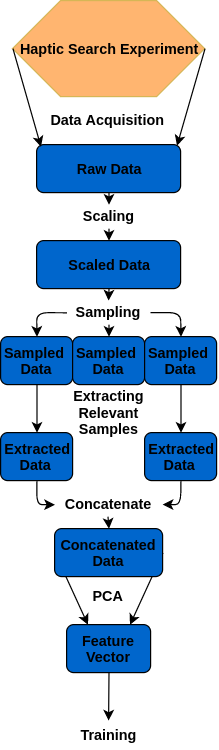
\includegraphics[scale]{Pipeline2}
	\makebox[\textwidth][c]{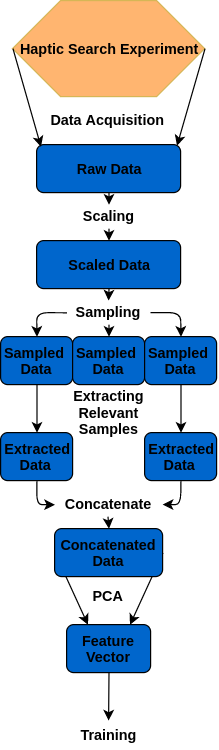
\includegraphics[scale=0.53]{Pipeline2}}
	\caption{Schematic representation of the complete Experimental Protocol}
	\label{pipeline}
\end{figure}

\subsection{Generating Training and Validation Set}
lol
%----------------------------------------------------------------------------------------
\section{Results and Discussion}
\subsection{E1}
\subsection{E2}
\subsection{E3}